\chapter{Introduction}

In this section we will write a short overview over themes and terms relevant for this study. Also we will introduce theory that both serve as a motivation and basis for the work seen later in this report.

\section{Background}
With the increasing demand of expected delivery from customers, many software development teams adopted agile methodologies as a development practice. Agile methodologies provides shorter feedback-loops than traditional waterfall and they allow teams to adapt both their products and working processes in short intervals. With the introduction of these methodologies a practice called ``Retrospective'' was introduced. Its roots based on reflective practices from organizational learning such as post-project reviews, experience reports and after action reviews. The purpose of the retrospective is allowing teams to look back at their last development phase and learn from it. Learning from the last period of time could provide useful knowledge that could be used to create improvement opportunities for future phases or projects. 

There have been several studies, \cite{Dingsoyr2004, Zedtwitz2002, bjornson2009, Hanssen2003, Dingsoyr2007, Bjarnason2012, Dingsoyr2003, Moe2001}, that investigates how to introduce and perform retrospectives. Derby and Larsen \cite{Larsen2006} even wrote a book on the subject. Literature describing the outcome of the retrospective however is a little bit sparse. Zedtwitz \cite{Zedtwitz2002} investigated organizational learning through post-project reviews in R\&D. Drury, Conboy and Power \cite{Drury2012} investigated the decision making in agile teams where retrospectives was one of the practices investigated. However we have not seen any studies that investigates the learning and outcome of retrospectives in a software development context. 

As the intervals between retrospectives are shorter than that of post-projects reviews we believe that the outcome and learning effects of the retrospective may differ from that of the post-project reviews. Based on this assumption we will conduct an empirical study that investigates the characteristics and learning effects of the retrospective of mature teams. Answering Dingsøyr and Dybå's call \cite{Dyba2008} for empirical studies into mature agile development teams. 

\section{Agile Development}
Agile development is a set of working methodologies that is prevalent in the software development industry \cite{Tessem2014}. Agile development focuses on high adaptability and customer communication, leading to supposedly higher effectiveness and lower costs. Scrum, Kanban and Extreme Programming are examples of popular agile methodologies that are used in today's software development industry. An ideal agile team has a high degree of self control and develop project goals through frequent communication with the customer, without being impeded by external processes. Some of the typical concepts included in an agile project environment are the daily meeting, retrospectives and iterations. The daily meeting is also called a stand up meeting and is typically a short meeting at the start of the day performed standing where team members talk about issues, obstacles and the plan for the day\cite{Moe2012}. This is by no means a full description of the agile development methodologies, but intended to give a context for the rest of the article.

\section{Retrospective}
Retrospectives, sometimes also called postmortems, are an activity that aim to improve learning within an organization. We will look at different retrospective definitions, some of the earlier academic work done on retrospectives and the characteristics of the retrospective in terms of retrospective outcome, processes and impediments in the following subsections.

\subsection{Retrospective Definitions}
There are several different definitions of retrospectives. Dingsøyr \cite{Dingsoyr2004} defines postmortem as: 

\begin{quote}
By a postmortem, we mean a collective learning activity which
can be organised for projects either when they end a phase or
are terminated. The main motivation is to reflect on what happened
in the project in order to improve future practise—for the
individuals that have participated in the project and for the organisation
as a whole. The physical outcome of a meeting is a postmortem report.
\end{quote}

Derby and Larsen \cite{Larsen2006} defines retrospectives in another way: 

\begin{quote}
A special meeting where the team gathers after completing an increment of work to inspect and adapt their methods and teamwork. Retrospectives enable whole-team learning, act as a catalysts for change, and generate action.
\end{quote}

We define retrospectives as the following:

\begin{quote}
	\textit{Retrospectives is a process that aims to facilitate shared learning within a team or an organization after a learning event, and such create a focus to improve current work practices or teamwork.}
\end{quote}

We say learning event as different teams holds retrospectives after different kinds of events. We list the kinds of retrospectives known to us in \autoref{table:retrospective-types}. For this paper our main focus will be related to what we call iteration retrospectives, which is the practice commonly used in SCRUM and Kanban. 

\begin{table}[!h]
	\begin{center}
		\caption{Types of retrospectives}
		\label{table:retrospective-types}
		\begin{tabular}{l l}
			\hline
			Retrospective Type & Description \\
			\hline
			Iteration Retrospective & Held after project iteration \\
			Project Retrospective & Held after a project ends \\
			Feature Retrospective & Held after the release of a feature \\
			Incidents Retrospective & Held after an incident \\
			Back-on-track retrospective & Held when work practices is failing \\
			\hline
		\end{tabular}
	\end{center}
\end{table}

\subsection{Retrospectives: Earlier Academic Work}
There have been several articles, conference papers, and experience reports on retrospectives or mentioning them as part of agile development.

Dingsøyr, Moe and Nytrø compared light-weight postmortem reviews against experience reports and found that the two provides different kind of experience. light-weight postmortem focuses on implmentation, administration, developers and maintence, while experience reports yield experience related to contract issues, design and technology. 

On the subject of retrospectives techniques several publications have been done. Stålhane, Dingsøyr, Hanssen and Moe\cite{Hanssen2003} compared two methods of semi-structured interviews and KJ-session and found that both may be applied to harvest knowledge. Bjarnason and Regnell\cite{Bjarnason2012} proposed the evidence-based timelines method as a way of conducting retrospectives. Bjørnson, Wang and Arisholm\cite{bjornson2009} compared the effectiveness of root-cause analysis against that of fishbone diagrams and found that root-cause analysis was more effective as the fishbone diagram limits the way issue were related to each other. Dingsøyr\cite{Dingsoyr2004} have written an article on the subject highlighting the purpose of the retrospective as well as discussing three possible approaches. Dølvik and Stålesen\cite{Dolvik2014} did a literature review on agile retrospectives and found that different techniques would fit different goals, and they found a lack of research considering follow-up on the issues identified during the retrospective. There also several experience reports on the subject, two of them Maham\cite{Maham2008}, Kinoshita\cite{Kinoshita2008}, which describes how to plan and facilitate retrospectives as well as describing different techniques. Finally Derby and Larsen\cite{Larsen2006} has as previously mentioned a book on the subject. 

Other work returns some different findings. Drury, Conboy and Power\cite{Drury2012} found in a study on obstacles to decision making in agile development teams that SCRUM-master prioritizes other tasks than follow-up on actions from retrospectives. They proposed that discussion on decision-making should be a part of the retrospective. And they found that some regarded the retrospective as a waste of time while others found it useful. Comparing to this Stålhane, Dingsøyr, Hanssen and Moe\cite{Hanssen2003} found that the participants of their case-study regarded the postmortem as useful. 

Zedtwitz\cite{Zedtwitz2002} identified several barriers for learning in post-project reviews in R\&D. Two psychological barriers were identified; inability to reflect and memory bias. Managerial barriers were time constraints and bureaucratic overhead. Epistemological barriers such as difficulty to generalize and tacitness of process knowledge were also identified by Zedtwitz. The last barriers were team-based and identified as reluctance to blame and poor internal communication. 

There are several publications mentioning retrospectives or directly addressing them, however most of these studies are related to how one should conduct retrospectives or the purpose of it. However we have not seen any studies addressing the value of the retrospective, which is in part why we have focused to conduct this case study. 

\subsection{Retrospective Outcome}
\label{intro:retro-outcome}
Conducting retrospectives should return some outcome for the teams doing them. Dingsøyr \cite{Dingsoyr2004} describes retrospectives as practice that could improve learning within an organization. Derby and Larsen \cite{Larsen2006} writes about the benefits of adapting and producing a better quality product and a better working life for team members. Drury, Conboy and Powers \cite{Drury2012} however states that the retrospective does not provide any real change for the teams conducting them. Throughout this study we will look at the outcome of the retrospective. We will mainly focus on the learning benefits, but we will also investigate the improvements the retrospective provides and the enthusiasm it brings. 

\subsubsection{Learning}
The learning benefits of conducting retrospectives can be viewed in several ways. Dingsøyr \cite{Dingsoyr2004} describes postmortems through learning as a process of conversion between tacit and explicit knowledge and learning through communities of practice. As a conversion process the participants employ learning through listening to others and thereby socialize and create their own tacit knowledge of the tacit knowledge told by others. Sharing your tacit knowledge externalizes the knowledge and makes it explicit. Through the communities of practice view Dingsøyr describes postmortem as an arena for individuals to contribute knowledge towards the community and for the community to reflect on practices. 

For this study we want to investigate which kind of learning occurs during the retrospective. To do that we will employ an organizational learning theory developed by Argyris and Schön \cite{Argyris1996}, called Organizational learning II that is described further in \autoref{intro:organizational-learning}. 

\subsubsection{Improvements}
Derby and Larsen \cite{Larsen2006} describes how retrospectives can improve team environments. It can help teams improve practices, handle issues and surface obstacles on a regular basis. Kinoshita \cite{Kinoshita2008} describes the importance of feedback that helps the team improve continuously through projects. Drury et. al. \cite{Drury2012} states that no real change occurs and that the team do not implement the improvement opportunities as short term tasks are prioritized over the long term ones. 

We have not seen any literature or studies on what improvements do occur in the retrospective. What topics are brought to the retrospective? What kind of decisions are made? And what improvements are actually implemented, and how is it implemented? We will investigate questions such as these and describe our findings throughout this report.

\subsubsection{Enthusiasm}
Derby and Larsen \cite{Larsen2006} states that teams are invested in the success of improving their work as the improvements are chosen by the teams themselves and not from upper management. Our own findings \cite{Dolvik2014} from previous literature review found that enthusiasm affect the retrospective. Recurring issues kills the enthusiasm and if the enthusiasm is low enough some might find that the retrospective is a waste of time, as also seen by Drury et. al. \cite{Drury2012}. We want to investigate this further through this study and focus on how the retrospective outcome is influenced by the enthusiasm from the team. 

\subsection{Retrospective Processes}
There are several approaches and methods on how to conduct a retrospective. We will look at two different approaches to conducting retrospectives, Dingsøyr's \cite{Dingsoyr2004} approach to postmortems and Derby and Larsen's Retrospective Structure \cite{Larsen2006}. After we have presented these we will present our own approach to retrospective practices and processes. 

\subsubsection{Dingsøyr's Approach to Postmortems}
\label{section:Dingsoyr-Approach-Introduction}
Dingsøyr \cite{Dingsoyr2004} discussed several considerations that companies should consider when conducting postmortem. These eight considerations is shown in \autoref{table:postmortem-approach}. 

\begin{table}[h]
	\begin{center}
		\caption{Dingsøyr's Approach to Postmortems}
		\label{table:postmortem-approach}
		\begin{tabular}{p{0.3\textwidth} p{0.7\textwidth}}
			\hline
			\textit{Approaches} & \textit{Description} \\
			\hline
			Requirements for a good postmortem process & Open dialogue, preventing critique of individuals and dominating people absorbing the meeting and maintaining a good atmosphere. \\
			Who to invite & Broad audience of project contributers, avoid external stakeholders. \\
			With or without homework & Homework can stimulate individual reflection, externalization, but require more time. Allowing participants to reflect during the meeting should deal with most important issues. \\
			Facilitator & External facilitator is recommended. \\
			Open or structured discussion & Open discussion can take a lot of time and dominating participants can absorb the discussion. KJ-method equally allows the participants to influence the discussion, however can be time-consuming to find names for issue-groups. \\
				With or without management & Not recommended, but with a strong facilitator project manager could be invited. \\
			Output & Describing report if project if goal is to spread knowledge. List of recommendations if improvements are only goal. \\
			Tacit or explicit knowledge & Small companies should share tacit knowledge, larger companies should codify it. \\
			\hline
		\end{tabular}
	\end{center}
\end{table}

The first consideration is requirements for a good postmortem process. Dingsøyr recommends having an open dialogue, where openness, patience, ability to listen, experimentation with new words and concepts, politeness, formation of a persuasive argument and courage are all present. Having a skilled process leader will help achieve this according to Dingsøyr. Also maintaining a good atmosphere is important. 

Who to invite is Dingsøyr's second consideration. He recommends inviting as many as possible that can contribute with knowledge for future projects to the postmortem. However external stakeholders are not recommended as this will move the focus to stakeholder relations. 

Dingsøyr's third consideration is homework before the retrospective. Homework can stimulate individual reflection and externalization, but it require more time. If the individuals instead are allowed to reflect during the postmortem the most important issues should be dealt with if there is enough participants. Another possible solution from Dingsøyr is to let the facilitator prepare before the retrospective. 

The fourth consideration is using a facilitator. He recommends using an external facilitator as it will help get a more thorough picture of the project.

Open or structured discussion is the fifth consideration. Dingsøyr describes how an open discussion easily can take a lot of time and be too limited in its focus in terms of number of issues. KJ-sessions are a structured discussion where every participant equally influence the discussion. There is also a risk in terms of time as finding names for groupings of issues may take some time. 

Including management in the postmortem is not recommended by Dingsøyr. The project manager should however be included if the facilitator is able to hinder him from taking a defensive position to the project. The reason he should be included is that he can provide a broader overview of the project compared to the participants. 

The output should be a list of recommendations or a report describing the project. If the goal is to spread knowledge in the company a short report on the project is appropriate. If the goal is only to improve a list of recommendations should suffice. 

The last consideration of Dingsøyr is whether the knowledge gained through retrospectives should remain tactic or made explicit. For small companies he recommends that they could easily share the tacit knowledge. For larger companies however he recommends using the resources needed to codify the knowledge and make it explicit. 

\subsubsection{Derby and Larsen's Retrospective Structure}
\label{section:Derby-Larsen-Structure}
Derby and Larsen \cite{Larsen2006} have structured the retrospective into five steps. The five steps can be seen in \autoref{table:retrospective-structure} and will be described below. 

\begin{table}[h]
	\begin{center}
		\caption{Derby and Larsen's Retrospective Structure}
		\label{table:retrospective-structure}
		\begin{tabular}{p{0.3\textwidth} p{0.7\textwidth}}
			\hline
			\textit{Step} & \textit{Description} \\
			\hline
			Set the stage & Reiterates the goal for the retrospective and helps participants focus on the work at hand. \\
			Gather data & Gathers a share picture of what happened during the last iteration. \\
			Generate Insights & Allows the team to see the big picture, and delve into root-causes, finding experiments and improvements. \\
			Decide what to do &  Provides structure and guidance for the team to plan experiments and actions. \\
			Close the retrospective & Helps the team retaining what they have learned from the retrospective. \\
			\hline
		\end{tabular}
	\end{center}
\end{table}

Setting the stage is the first step described by Derby and Larsen. The purpose is to help the participants focus on the work at hand. The step include establishing the purpose, method and timeframe for how the retrospective is planned. It also includes establishing a safe environment where the participants can have a challenging discussion. Creating a working agreement is recommended so the retrospective can remain a civil arena for collaboration. 

The second step is gathering data. Gathering data helps create a shared picture of what happened, expanding the participants individual perspective. It is recommended starting with hard data such as events, metrics, completion rates and so on. Afterward feelings should be gathered so that one can get an impression on which issues is most important. Gathering feelings also helps avoiding motivation loss or venting situations according to Derby and Larsen.

Generate insights is the third step recommended by Derby and Larsen. The purpose is to help the team generate solutions and experiments that will improve the team's current practices. It is stated that the first solution is most likely incorrect and that the team should maintain a root-cause focus. 

The fourth step proposed by Derby and Larsen is deciding what to do. After the former steps a list of possible experiments and improvements should have been devised. The purpose of this step is to help guide the team plan to implement the changes to the next iteration. It is recommended that one assigns individuals to the actions as it won't get done if just the team is assigned to it. 

Closing the retrospective is the final step in Derby and Larsen's structure for conducting retrospectives. They recommend ending the retrospective decisively to avoid the participants energy dribbling away. It is also recommend using just a couple of minutes giving feedback on the retrospective before ending it. 

\subsubsection{Own Framework}
\label{subsubsec:own-framework}
Derby and Larsen describes how to conduct a retrospective and Dingsøyr investigates different considerations one should employ before conducting a retrospective. None of them takes into considerations the outcome of the retrospective. Through our earlier studies \cite{Dolvik2014} we found that the retrospective could be split into three parts: Before, During and After the retrospective, which is shown in \autoref{figure:retro-barebone}. By including the after retrospective part into the framework we are able to describe the outcome of the retrospective practice which is missing from Dingsøyr's and Derby and Larsen's processes. We will describe each of the three parts and how the framework aligns with Derby and Larsen's and Dingsøyr's processes below. 

\begin{figure}[!h]
	\centering
	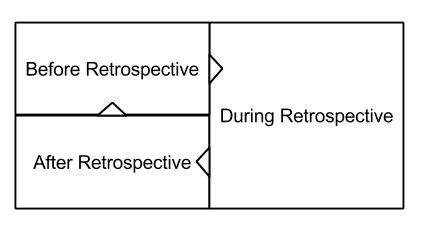
\includegraphics[width=\textwidth, keepaspectratio]{figures/retro-barebone.png}
	\caption{Own Framework for Retrospectives}
	\label{figure:retro-barebone}
\end{figure}

Before the retrospective, preparation is required no matter how one conducts the retrospective. At the very least one must have a wish to improve and invite the participants for the retrospective. Depending on how one want to conduct the retrospective one could also gather data or evidence beforehand and declare a focus for the retrospective. The participants are also required to have some experiences that could be used as input for the retrospective. During the preparations for the retrospective Dingsøyr's considerations could be a valuable thing for the facilitator to investigate. It can help improve the retrospective and maintain the focus the facilitator or team wishes to have for the retrospective. 

During the retrospective one wish to reflect about the past to find improvement opportunities and learn. Several techniques are recommended by literature such as KJ-sessions, timelines, evidence-based timelines, root-cause analysis and open discussion. The focus is to learn from past work and find ways to improve in an open arena together in the team. Derby and Larsen's five steps is one way to arrange the retrospective meeting and will help maintain a focus for the retrospective. 

Finally we have after the retrospective where the outcome, which is described in \autoref{intro:retro-outcome}, of the retrospective should be apparent. This period lasts from the retrospective meeting ends until the next one begins. During this time experiments and improvements should be implemented. This should result in some learning which can be brought for the next retrospective and some enthusiasm as the work-life of the team improves. We have not seen any framework that consider this phase of the retrospective in any literature previously and is one of the reasons this framework is devised. 

Our framework is not exclusive with the existing frameworks found in previous literature. Dingsøyr's list of recommendations and Derby and Larsen's process of conducting retrospective are both able to exist within this framework where one consider the retrospective cycle. In \autoref{figure:retro-basis} we have displayed the framework and its relation to previous processes and the expected outcome of the retrospective practice. We will use this framework to describe the results throughout this study.

\begin{figure}[!h]
	\centering
	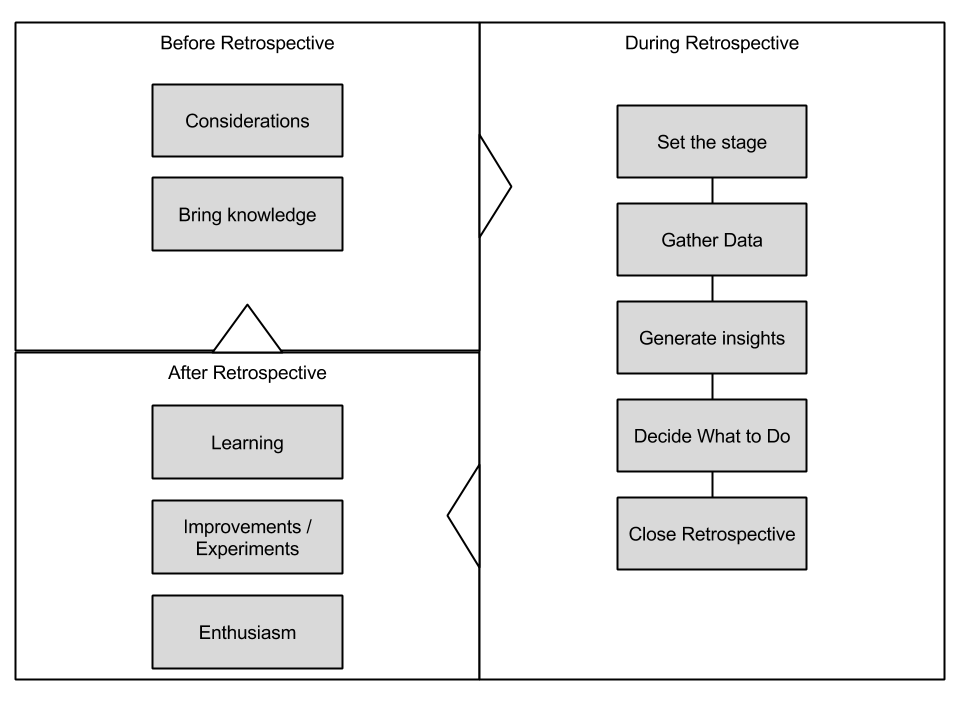
\includegraphics[width=\textwidth, keepaspectratio]{figures/retro-basis.png}
	\caption{Own framework for retrospectives with existing recommendations from previous literature.}
	\label{figure:retro-basis}
\end{figure}

\subsection{Retrospective Impediments}
Retrospective practices is a simple process that aims to inspire learning and create improvement opportunities for teams conducting them, however it suffers from impediments. Not a single company was satisfied with their after project reviews was one of the results Keegan and Turner \cite{Keegan2000} found after conducting a survey. Zedtwitz investigates organizational learning through post-project reviews and finds eight barriers for learning in the practice. Drury, Conboy and Power \cite{Drury2012} finds six obstacles to decision making that hinder improvements to be implemented from the retrospective. We will describe Zedtwitz barriers and Drury's et. al. obstacles below and through this study impediments facing the retrospective will be investigated and the results described. 

\subsubsection{Zedtwitz Barriers}
In an article Zedtwitz identifies four areas with a total of eight barriers that act as a resistance to learning through post-project reviews ~\cite{Zedtwitz2002}. These four areas are psychological, team based, managerial and epistemological. An overview over the areas and their related barriers can be seen in summarized \autoref{table:zedwitz-barriers} based on a figure from Zedtwitz's article. 

\begin{table}{!h}
	\begin{center}
	\caption{Zedtwitz\cite{Zedtwitz2002} Barriers}
	\label{table:zedwitz-barriers}
	\begin{tabular}{p{0.5\textwidth} p{0.5\textwidth}}
	\hline
	Area & Barriers \\
	\hline
	Psychological & Memory bias \\ 
	& Inability to reflect \\
	Managerial & Time constraints \\
	& Bureaucratic overhead \\
	Team-based & Reluctance to blame \\
	& Poor internal communication \\
	Epistemological & Difficult to generalize \\
	& Tacitness of process knowledge \\
	\hline
	\end{tabular}
	\end{center}
\end{table}

\paragraph{Psychological barriers}
The memory bias barrier is based on the human tendency to place a subjective importance on our experiences, for example Zedtwitz mentions an over emphasis on negative experiences, as these are easy to remember. 

An inability to reflect is the second psychological barrier, this might be caused by a belief that past experiences are irrelevant as circumstances change. It was found that often managers are unaware of the past when it came to actions and rationale.

\paragraph{Team-based Shortcomings}
The first team based barrier is a reluctance within the team to blame, leading to deflection of blame from the real issues. This might be as a result of an aversion to accepting personal failure or fear of embarrassment. 

Poor team internal communication is the second barrier, a team might intentionally hide information to gain an advantage over other teams when it comes to performance or promotions. Other factors might be physical distances making communication harder.

\paragraph{Epistemological}
The first barrier is a failure to generalize experiences from a specific context can lead to no experiences being transferable to future projects. 

The second barrier is the tacitness of knowledge. The barrier addresses that knowledge cannot be shared easily. And reports or similar mediums might not reflect all the knowledge.

\paragraph{Managerial Constraints}
Time constraints are a barrier that might lead to retrospectives not being held. This is a result of time being considered critical and retrospection and reflection being down prioritized. 

The last barrier is bureaucratic overhead, it might be hard to justify a retrospective session to bureaucracy because of a lack of immediately profitable output.

\subsubsection{Effective Decision Making}
The term decision making refers to the process of a team making a decision that impacts the team or its environment. In their article Moe et. al. ~\cite{Moe2011} talk about three layers of decision making, operational, tactical and strategic. These levels are described in \autoref{table:decision-making-levels}. 

\begin{table}[h]
	\begin{center}
		\caption{Decision making levels}
		\label{table:decision-making-levels}
		\begin{tabular}{l l}
			\hline
			Decision level & Description \\
			\hline
			Operational & Day to day operations. \\
			Tactical & Resource management.\\
			Strategic & Goal and objectives, often long term. \\
			\hline
		\end{tabular}
	\end{center}
\end{table}

Software development can be both routine and non-routine, and the decisions that relate to this is rational decision making and non-bounded decision making. Where rational decision making is assuming that decision makers have complete information and possible solutions, and can therefore choose the decision most suitable. Rational decision making is often related to routine decisions. When goals are changing it makes more sense to talk about non-routine decisions, and these can be described within the bounded rationality model. In this model the decision maker is restricted, in information and problem types. 

Drury et. al. ~\cite{Drury2012} discusses obstacles to decision making present in agile software development teams. They specifically describes how an iteration retrospective can result in decision making that leads to improvement of future performance. However this is not necessarily the case as some retrospectives can become a place to vent frustration instead of productive decision making. A summary on the barriers identified by Drury et. al. can be found in \autoref{table:Drury-barriers}

\begin{table}[h]
	\begin{center}
		\caption{Drury barriers}
		\label{table:Drury-barriers}
		\begin{tabular}{ p{0.5\textwidth} | p{0.5\textwidth}}
			\hline
			Barrier & Description \\
			\hline
			Team members unwilling to commit and relying on scrum master & A lack of commitment in a team leading to the burden being put on the coach, scrum master or managers. \\
			Conflicting priorities & A team might have multiple priorities or customers that lead to difficultly setting priorities \\
			Decisions based on unstable staff availability & If people are moved to another project this can lead to problems with the strict estimations typical in an agile project \\
			Not implementing decisions or relying on others for decisions & The failure to implement an agreed upon decision, or expecting someone else to do it leads to decisions falling flat \\
			Not taking ownership of decisions & Teams failing to take ownership of their decisions leading to decision implementation being lackluster, often as a result of a decision not being designated to someone responsible\\
			Collaboration stops experts from making decisions & The empowerment of the team can lead to individual experts not having the control over decisions they had previously \\
			\hline
		\end{tabular}
	\end{center}
\end{table}

\clearpage

\section{Organizational Learning}
\label{intro:organizational-learning}
Organizational learning is in simple terms how an organization is able to acquire, store and utilize knowledge existing within an organization. In a more academic setting we can use Argyris and Schön's definition \cite{Argyris1996} for organizational learning: 

\begin{quote}
	``Organizational learning occurs when individuals within an organization experience a problematic situation and inquire into it on the organization's behalf. They experience a surprising mismatch between expected and actual results of action and respond to that mismatch through a process of thought and further action that leads them to modify their images of organization or their understandings of organizational phenomena and to restructure their activities so as to bring outcomes and expectation into line, thereby changing organizational theory-in-use. In order to become organizational, the learning that results from organizational inquiry must become embedded in the images of organization held in its members' minds and/or in the epistemological artifacts (the maps, memories, and programs) embedded in the organizational environment. ''
\end{quote}

Organizational learning can be applied to groups of people over different sizes. One can use it to analyze huge organizations consisting of many actors in different roles, or small groups of people working closly together. For this research we are going to apply the organizational learning at an agile development team. 

Different types of frameworks exist for organizational learning. Levitt and March uses a framework that sees learning in organizations as encoding inferences from history into routines that guide behavior \cite{Levitt1988}. The retrospective is a process of shared learning for an agile development team learning from the last iteration of development. Investigating learning using this framework won't yield much as the retrospective already is seen as a collective learning activity \cite{Dingsoyr2004}. 

Argyris and Schön \cite{Argyris1996} uses two different models to determine how an organization learns through individuals, Model I and Model II. As agile teams often are limited to a close group of individuals we will apply Argyris and Schön's models. To understand these models we first need to investigate two types of learning: Single-loop learning and double-loop learning. Further in this section we will explain these types of learning as well as Model I and Model II. We have borrowed \autoref{table:model-I}, \autoref{table:model-II}, \autoref{table:social-virtues} from Argyris and Schön's ``Organizational learning II: Theory, Method and Practice''\cite{Argyris1996} and they provide a quick overview of the two models as well as the social virtues that differs between them. We will also look at Triple-loop learning as it is the concept of learning about learning. 

\subsection{Single-loop}
Single-loop learning is a type of learning defined by Argyris and Schön. It consist of a single-feedback loop that finds an error and a way to fix this problem. Argyris and Schön \cite{Argyris1996} defines single-loop as: 

\begin{quote}
``By single-loop learning we mean instrumental learning that changes strategies of action or assumptions underlying strategies in ways that leave the value of a theory of action unchanged.

... In such learning episodes, a single feed-back loop, mediated by organizational inquiry, connects detected error - that is, an outcome of action mismatched to expectations and, therefore, surprising - to organizational strategies of action and their underlying assumptions. These strategies of action and their underlying assumptions. These strategies or assumptions are modified, in turn, to keep organizational performance within the range set by existing organizational value and norms. The values and norms themselves ... remain unchanged. 
''
\end{quote}

An example of single-loop learning from software development could be finding a bug, find a solution to fix it and then fix it. The single-loop learning would here be learning the solution and fixing the bug. We have provided a basic illustration of single-loop learning in \autoref{figure:single-loop}.

\begin{figure}[!h]
	\centering
	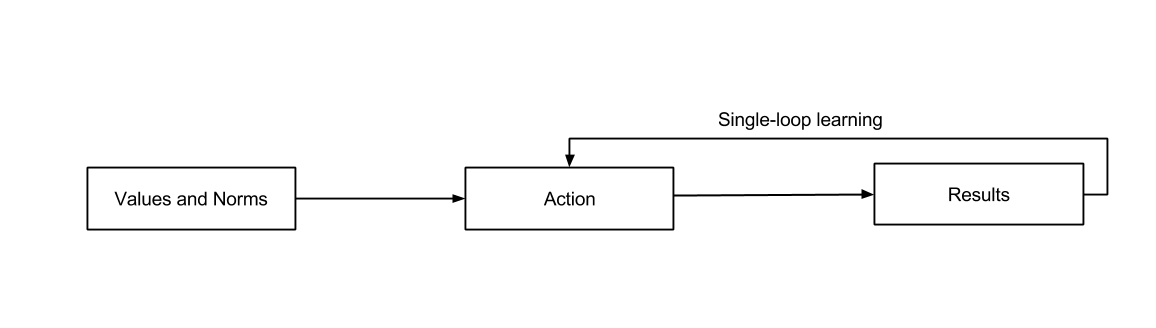
\includegraphics[width=\textwidth, keepaspectratio]{figures/Single-loop.png}
	\caption{Single-loop learning visualization, based on Argyris and Schön's single-loop learning \cite{Argyris1996}.}
	\label{figure:single-loop}
\end{figure}

\subsection{Double-loop} % (fold)
\label{sub:double_loop}
Double-loop learning is a type of learning where one asks whether the underlying factors that influence the actions and results is sufficient.
One might say that one understands the root-cause for the issue. 
Argyris and Schön defines double-loop learning as: 

\begin{quote}
``By double-loop learning, we mean learning that results in a change in the values of theory-in-use, as well as in its strategies and assumptions. The double loop refers to the two feedback loop that connect the observed effects of actions with startegies and values server by strategies. Strategies and assumptions may change concurrently with, or as a consequence of, change in values. Double-loop learning may be carried out by individuals, when their inquiry leads to change in the values of their theories-in-use or by organizations, when indivduals inquire on behalf of an organization in such a way as to lead to change in the values of organization theory-in-use. ''
\end{quote}

This type of learning can be shown in our bug example. If the developers who earlier found and fixed a bug did a root-cause analysis on the issue they could get several results indicating that underlying factors are not sufficient for the current state of development team. One underlying factor could be weak specification description requiring the team to rethink and restructure how they develop specifications. Another reason could be that the knowledge for the system is not good enough with the developers indicating a knowledge-gap in the team and considerations for the state of the team may be required. 

For this research we use the term double-loop learning when the influences for the issue is understood and change occurs as a results of this. A simple figure of double-loop learning can be seen in \autoref{figure:double-loop}

\begin{figure}[!h]
	\centering
	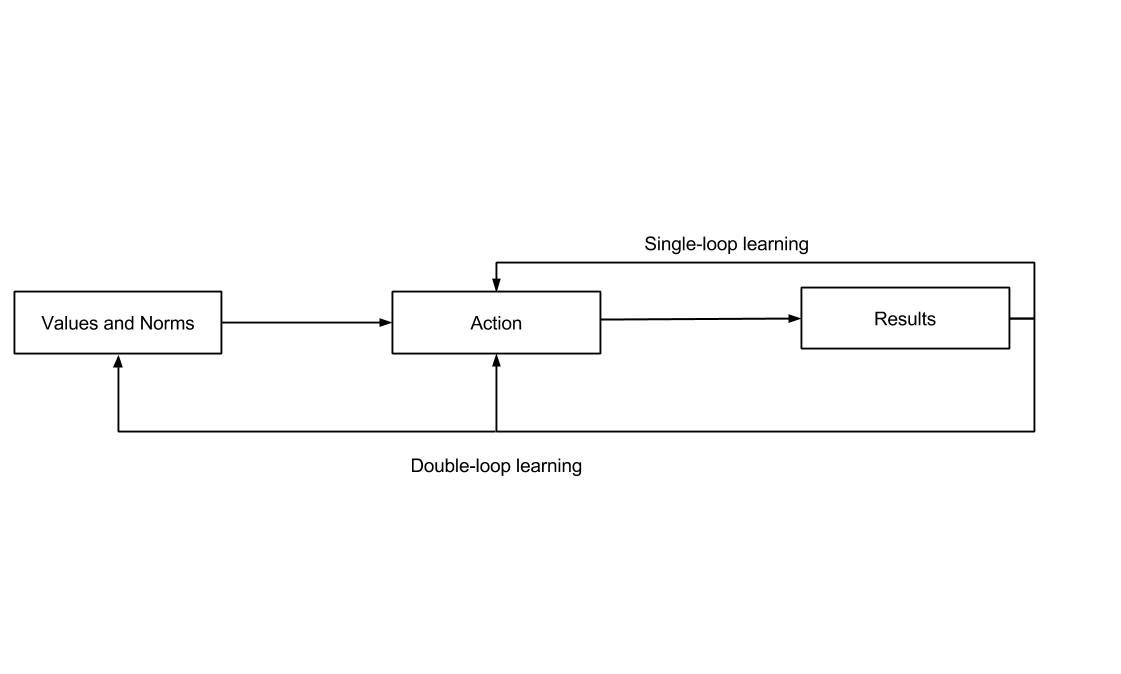
\includegraphics[width=\textwidth, keepaspectratio]{figures/double-loop.png}
	\caption{Double-loop learning visualization, based on Argyris and Schön's double-loop learning \cite{Argyris1996}}
	\label{figure:double-loop}
\end{figure}

% subsection triple_loop (end)
\subsection{Model I} % (fold)
\label{sub:model_i}
Argyris and Schön \cite{Argyris1996} describes a learning system called Organizational learning I, which theory-in-use is described as Model I. As organizational learning I is an employed learning system that can be defined by different actions and implementations we will instead go into the theory-in-use, Model I, as these systems employ them.

Argyris and Schön \cite{Argyris1996} describes Model I through its governing variables. We will go through each of them along with the actions strategies, consequences for behavioral world and consequences for learning, effectiveness that follows of the different governing variables that actors try to satisfy. 

The first governing value described is defining goals and trying to achieve them. This leads to the action strategies of designing and managing the environment unilaterally. The behavioral consequences are that the actor gets seen as defensive, inconsistent, incongruent, controlling, fearful of being vulnerable, withholding feelings, overly concerned about self and others, or under-concerned about others. For the effectiveness and learning the consequences are that the actor is self-sealing and the longterm effectiveness is decreased. 

Maximize winning and minimize losing is the second governing variable that the actors in an organization try to satisfy. The actions strategies for this governing value is that the actor takes ownership and control of a task. This results in a defensive interpersonal and group relationship where the actor wants the rest of the group to see things his way and little help could be a result of this. For terms of learning this will provide single-loop learning as the output of the task is more important than the task itself. 

The third governing value for the actors in this kind of learning model is minimizing generating or expressing negative feelings. The action strategy that follows is that the actors wishes to protect themselves using defensive actions such as blaming, stereotyping and suppressing feelings. The consequences for the behavioral world is defensive norms within the organizations. Rivalry, lack of external commitment and mistrust are examples of such norms. For the learning consequences of this value little theories will be tested publicly prohibiting double-loop learning in the organization. However there will still be much testing of theories with the individuals, however this knowledge will not reach the organization. 

Being rational is the fourth and final governing variable for Argyris and Schön's Model I theory-in-use for the learning organization. Being rational provides the action strategy of protecting others from being hurt resulting in actions like withholding information, creating censoring rules that can censor information and behavior. This returns the same consequences for the behavioral world, learning and effectiveness as described above. 

Through the governing values of Model I the actors within the organization prohibits double-loop learning. The organization creates a win or loose situation between the actors leading to withholding of information, mistrust between the actors and little testing of current norms or values. This again provides competition instead of collaboration and thus have a negative impact on the learning and effectiveness of the organization. Model I is further described by Argyris and Schön as the different elements of the model interact in complex ways. This can be read about in ``Organizational learning II: Theory, Method and Practice'' \cite{Argyris1996}.

\begin{sidewaystable}[!h]
	\begin{center}
	\caption{Theory-in-use of Organizational learning I borrowed from ``Organizational learning II: Theory, Met hod and Practice'' by Argyris and Schön \cite{Argyris1996}}
	\label{table:model-I}
	\makebox[\textwidth]{%
		\begin{tabular}{ p{0.25\textwidth} p{0.25\textwidth} p{0.25\textwidth} p{0.25\textwidth} }
		\multicolumn{4}{l}{\textit{Model I Theory-in-Use}} \\
		\hline
		\textbf{Governing Variables} & \textbf{Action Strategies} & \textbf{Consequences for Behavioral World} & Consequences for Learning, Effectiveness \\
		Define goals and try to achieve them. & Design and manage the environment unilaterally (be persuasive, appeal to larger goals, etc.) & Actor seen as defensive, inconsistent, incongruent, controlling, fearful of being vulnerable, withholding of feelings, overly concerned about self and others, or under-concerned about others. & Self-sealing. 

		Decreased Long-term effectiveness. \\
		Maximize winning and minimize loosing. & Own and control the task (claim ownership of the task, be guardian of the definition and execution of the task). & Defensive interpersonal and group relationship (depending on actor, little help to others). & Single-loop learning. \\
		Minimize generating or expressing negative feelings. & Unilaterally protect yourself (speak in inferred categories accompanied by little or no directly observable data, be blind to impact on others and to incongruity; use defensive actions such as blaming, stereotyping, suppressing feelings, intellectualizing). & Defensive norms (mistrust, lack of risk taking, conformity, external commitment, emphasis on diplomacy, power-centered competition and rivalry). & Little testing of theories publicly. 

		Much testing of theories privately. \\
		Be rational. & Unilaterally protect others from being hurt (withhold information, create rules to censor information and behavior, hold private meetings). & & \\
		\hline
		\end{tabular}
	}
	\end{center}
\end{sidewaystable}

% subsection model_i (end)
\subsection{Model II} % (fold)
\label{sub:organizational_learning_ii}
The second model described by Argyris and Schön is the theory-in-use for organizational learning II systems called Model II. While Model I is creating a win-loose relationship between the actors resulting in actors trying to control the environment, Model II instead invites the actors to confront each others views and emotions. This is creating an environment for double-loop learning where the actors strive to get the most complete understanding of their environment and adapt this. 

There are three governing values for Model II according to Argyris and Schön: Valid information, Free and informed choice and Internal commitment to the choice and constant monitoring of its implementation. 

The three governing values give primarily four behavioral strategies. ``Designing situations where participants can be origins of action and experience high personal causation'' is one the strategies according Argyris and Schön. Another of these strategies is that the group of actors jointly control the tasks. This provides an environment where face-saving for the individual should not be needed and thus facilitates open and clear communication between the different actors. This again is connected to the third action strategy that is ``Protection of self is a joint enterprise and oriented towards growth''. The three governing values also provide an environment of bilateral protection towards others. 

There are several consequences for the behavioral world following the governing values and behavioral strategies for Model II. The first one is that actors within the organization act less defensively than in Model I systems and is experienced as minimally defensive. The second consequence is the same as the first one except that it relates to the relationship between the different individuals in the organization. The group dynamics and interpersonal relationships will be minimally defensive. As an organization approaches the practices that supports the three governing values learning-oriented norms will start appearing in the organization as a consequence. The final consequence Argyris and Schön describe is high freedom of choice, internal commitment and risk taking within the organization. 

As for the consequences on learning Model II will support double-loop learning. Disconfirmable processes and frequent public testing of theories will both support double-loop learning. As the defensive stance of the actors and relationships are minimized Model II practices will advocate and allow the organization to test their current theories on how their organization is performing, allowing for double-loop learning. 

As described by Argyris and Schön the Model II will in the long term increase effectiveness within an organization. Through facilitating collaboration rather than competition, allowing testing of the currently perceived world and norms and allowing experimentation the Model II allows double-loop learning. Being able to adapt the organization through double-loop learning will in the long term increase the effectiveness. 

Finally the Modell II theory-in-use is not a goal one can achieve as described by Argyris and Schön. Instead it is a focus one can work against, as the nature of the Modell II and double-loop learning is always to challenge the current world for better one can never achieve the ideal world as this world will always be able to change and improve. 

\begin{sidewaystable}[!h]
	\begin{center}
	\caption{Theory-in-use of Organizational learning II borrowed from ``Organizational learning II: Theory, Method and Practice'' by Argyris and Schön \cite{Argyris1996}}
	\label{table:model-II}
	\makebox[\textwidth]{%
		\begin{tabular}{p{0.2\textwidth} p{0.2\textwidth} p{0.2\textwidth} p{0.2\textwidth} p{0.2\textwidth}}
		\multicolumn{5}{l}{\textit{Model II Theory-In-Use}}\\
		\hline
		\textbf{Governing Variables for Action} & \textbf{Action Strategies} & \textbf{Consequences of Behavioral World} & \textbf{Consequences on Learning} & \textbf{Consequences on effectiveness} \\
		\hline
		\begin{itemize}[leftmargin=*]
			\item[] Valid information
			\item[] Free and informed choice 
			\item[] Internal commitment to the choice and constant monitoring of its implementation
		\end{itemize}
		&
		\begin{itemize}[leftmargin=*]
			\item[] Design situations where participants can be origins of action and experience high personal causation
			\item[] Task is jointly controlled
			\item[] Protection of self is a joint enterprise and oriented toward growth
			\item[] Bilateral protection of others
		\end{itemize}
		&
		\begin{itemize}[leftmargin=*]
			\item[] Actor experienced as minimally defensive
			\item[] Minimally defensive interpersonal relations and group dynamics
			\item[] Learning-oriented norms
			\item[] High freedom of choice, internal commitment, and risk taking 
		\end{itemize}
		& 
		\begin{itemize}[leftmargin=*]
			\item[] Disconfirmable processes
			\item[] Double-loop learning
			\item[] Frequent public testing of theories
		\end{itemize}
		& Increased long-term effectiveness \\
		\hline
		\end{tabular}
	}
	\end{center}
\end{sidewaystable}

\begin{table}[!h]
	\begin{center}
	\caption{Social Virtues of Model I and Model II borrowed from ``Organizational learning II: Theory, Method and Practice'' by Argyris and Schön \cite{Argyris1996}}
	\label{table:social-virtues}
	\makebox[\textwidth]{%
		\begin{tabular}{ p{0.5\textwidth}  p{0.5\textwidth} }
		\textit{Model I Social Virtues} & \textit{Model II Social Virtues} \\
		\hline
		\textbf{Help and Support} & \\
		Give approval and praise to others. Tell others what you believe will make them feel good about themselves. Reduce their feelings of hurt by telling them how much you care and, if possible, agree with them that the others acted improperly. & Increase the other's capacity to confront their own ideas, to create a window into their own mind, and to face the unsurfaced assumptions, biases, and fears that have informed their actions toward other people. \\ 
		\\
		\textbf{Respect for Others} & \\
		Defer to other people; do not confront their reasoning or actions. & Attribute to other people of high capacity for self-reflection and self-examination without becoming so upset that they lose their effectiveness and their sens of self-responsibility and choice. Keep testing this attribution. \\
		\\
		\textbf{Strength} & \\
		Advocate your position in order to win. Hold your own position in the face of advocacy. Feeling vulnerable is a sign of weakness. & Advocate your position and combine it with inquiry and self-reflection. Feeling vulnerable while encouraging inquiry is a sign of strength. \\
		\\
		\textbf{Honesty} & \\
		Tell other people no lies, or tell others all you think and feel. & Encourage yourself and other people to make public tests of their ability to say what they know yet fear to say. Minimize what would otherwise be subject to distortion and cover-up of the distortion. \\
		\\
		\textbf{Integrity} & \\
		Stick to your principles, values, and beliefs. & Advocate your principles, values, and beliefs in a way that invites inquiry into them and encourages other people to do the same. \\
		\hline
		\end{tabular}
	}
	\end{center}
\end{table}

% subsection organizational_learning_ii (end)
% subsection double_loop (end)
\subsection{Triple-loop} % (fold)
\label{sub:triplloop}
The term triple-loop learning has been used in different ways as highlighted by Tosey, Visser and Saunders \cite{Tosey2011}. Triple-loop learning can be referring to both triple-loop learning and deutoro-learning. For this work we are going to stick with triple-loop learning. Tosey, Visser and Saunders performed a critical review of the triple-loop learning concept and finds that three concepts have been widely used in academic literature. 

The first concept they investigate is a form for learning above double-loop learning that addresses some learning in a level above the governing variable of double-loop learning. Tosey et. al. finds that this concept seem to be poorly defined, imprecise and unfounded in the way it is used. 

The second concept describes triple-loop learning as a form for meta-learning, a form of learning not above single-loop and double-loop, but rather beside. Learning about learning is a simple description. Tosey et. al. finds that this concept is a renaming of deutoro-learning and raises the question if this renaming is needed. 

The final concept connects triple-loop learning to Bateson's Learning III, which can be read about in ``Gregory Bateson on deutero-learning and double bind: A brief conceptual history'' by Visser \cite{Visser2003}. This concept relates to a type of learning that is non-instrumental and exists beyond language. Tosey et. al. finds that the literature that uses this concept have not been conducting a comprehensive working-through of Bateson's Theory. 

For our research we are going to use the second concept, where triple-loop learning is regarded as a kind of meta-learning. We define triple-loop learning as the learning about learning, where one organization is able to understand the learning processes occurring within the company and learn from these. A simple figure is provided in \autoref{figure:triple-loop}.

As an example of triple-loop learning we again turn to the bug example used earlier. After understanding both how to solve the bug and the influences which made the bug occur, the development team can investigate their learning process, by for an example retracing their steps from noticing the issue until they have understood the influences which made the bug occur. Along the way they may be able to learn how to investigate future problems or change the way they already learn through their given processes. 

\begin{figure}[!h]
	\centering
	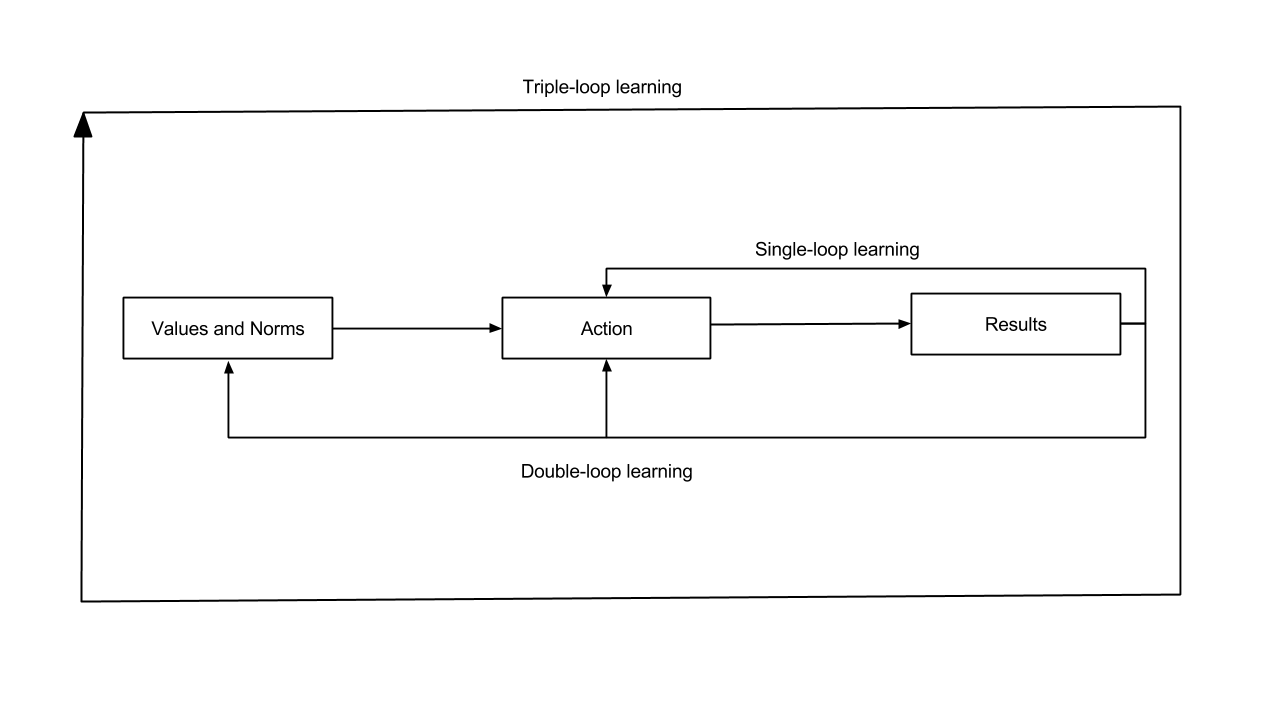
\includegraphics[width=\textwidth, keepaspectratio]{figures/triple-loop.png}
	\caption{Triple-loop learning visualization, based on Argyris and Schön's deutoro-learning as described by Tosey et. al. \cite{Tosey2011}}
	\label{figure:triple-loop}
\end{figure}

\clearpage 

\section{Terminology}
In this section we have an oversight of the terminology used in this thesis, this is by no means a comprehensive discussion of the terms, but meant to be a reference of words and ideas that might not necessarily be self explanatory or common knowledge. Our terminology can be found in \autoref{table:thesis-terminology}.

\begin{table}
	\begin{centering}
		\label{table:thesis-terminology}
		\caption{Thesis terminology}
		\begin{tabular}{ p{0.2\textwidth} p{0.2\textwidth} p{0.6\textwidth}}
			\hline
			\textit{Term} & \textit{Other terms} & \textit{Description} \\
			\hline
			Retrospective & Post mortem, after action review, post-project review & A process that aims to facilitate shared learning within a team or an organization after a learning event, and such create a focus that aims to improve the current work practices or teamwork.  \\
			Sprint & Iteration, release cycle, project phase & A time period in a project, often ending at a set date or goal \\
			Shared mental models & & Group level thought processes and actions, commonality in understanding enabling consensus and attaining goals \\
			Shared mental model accuracy & & The degree with which a team's mental model matches objective measurements \\
			Shared mental model similarity & & The degree with which the team member's mental models are similar \\
			Organizational Learning & & Academic field of how organizations or teams achieve learning. \\
			Single loop learning & Tuning, quick-fix & An action aimed at improving a process or fixing a problem, often immediately \\
			Double loop learning & Root-cause analysis & An action designed to improve a problem or process by fixing an underlying influence \\
			Theory-in-use & & Value, action strategies and norms that act as a theory for some process. \\
			Model I & Organizational learning I & The theory-in-use for a learning system of organizational learning I. \\
			Model II & Organizational learning II & The theory-in-use for a learning system of organizational learning II. \\
			\hline
		\end{tabular}
	\end{centering}
\end{table}
\clearpage
